\subsection{Escalas de tiempo}

\begin{frame}[t]
\frametitle{\subsecname}

\begin{definition}
Una escala de tiempo es un conjunto arbitrario cerrado no vacío $\mathds{T}\subseteq\mathds{R}$ bajo la topología estándar de $\mathds{R}$.
\end{definition}

\begin{example}
	\begin{itemize}
		\item $\left[1,2\right]$, $\mathds{R}$ y $\mathds{N}$ \alert{son escalas de tiempo}.
		\item $\left[a,b\right)$, $\left(a,b\right]$ y $\left(a,b\right)$ \alert{no son escalas de tiempo} si $a<b$.
		\item El conjunto \[ \left\{1,2,3\right\}\cup\left[4,5\right]\cup\left\{11,12,13\right\} \] \alert{es una escala de tiempo}.
	\end{itemize}
\end{example}

\begin{alertblock}{Ejercicio}
Pruebe que los siguientes conjuntos son escalas de tiempo.
	\begin{multicols}{2}
		\begin{enumerate}[topsep=0pt]
			\item $h\mathds{Z}\coloneqq\left\{hk:k\in\mathds{Z}, h\in\mathds{R}\right\}$.
			\item $\mathds{P}_{a,b}\coloneqq\bigcup_{k=0}^{\infty}\left[k\left(a+b\right),k\left(a+b\right)+a\right]$, $a>0$.
			\item $\overline{q^{\mathds{Z}}}\coloneqq\left\{q^{k}:k\in\mathds{Z}\right\}\cup\left\{0\right\}$, $q>1$.
			\item $\mathds{N}^{n}_{0}\coloneqq\left\{k^{n}:k\in\mathds{N}_{0}\right\}$, $n\in\mathds{N}$.
			\item $\left\{H_{n}:n\in\mathds{N}_{0}\right\}$, donde $H_{n}$ son los llamados \emph{números armónicos} definidos por $H_{0}=0$ y $H_{n}=\sum_{k=1}^{n}\frac{1}{k}$, $\forall n\in\mathds{N}$.
			\item $\mathcal{C}\coloneqq\bigcap_{n=0}^{\infty}K_{n}$, donde $K_{0}=\left[0,1\right]$. $\mathcal{C}$ es el \emph{conjunto de Cantor}.
		\end{enumerate}
	\end{multicols}
\end{alertblock}
\end{frame}

\begin{frame}

\begin{definition}
Para $t\in\mathds{T}$, definimos el \textbf{operador salto posterior} $\sigma\colon\mathds{T}\rightarrow\mathds{T}$ por \[ \sigma\left(t\right)\coloneqq\inf\left\{s\in\mathds{T}:s>t\right\}. \] Note que $\sigma\left(t\right)\geq t$ para cualquier $t\in\mathds{T}$.
	\end{definition}

\begin{definition}
Para $t\in\mathds{T}$, definimos el \textbf{operador salto anterior} $\rho\colon\mathds{T}\rightarrow\mathds{T}$ por \[ \rho\left(t\right)\coloneqq\sup\left\{s\in\mathds{T}:s<t\right\}. \] Note que $\rho\left(t\right)\leq t$ para todo $t\in\mathds{T}$.
\end{definition}

\begin{definition}
La función \textbf{granicidad} $\mu\colon\mathds{T}\rightarrow\left[0,+\infty\right)$ es definido por \[ \mu\left(t\right)=\sigma\left(t\right)-t,\quad\forall t\in\mathds{T}. \]
\end{definition}
%función granicidad minimal $\mu_{\ast}\colon\mathds{T}\rightarrow\mathds{R}$ por \[ \mu_{\ast}\left(s\right)=\inf_{\tau\in\left[s,\infty\right)\cap\mathds{T}}\mu\left(t\right). \]
\begin{figure}[H]
	\centering
	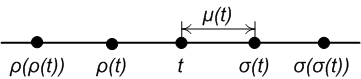
\includegraphics[width=0.4\paperwidth]{operators}
	%\caption{Los operadores $\sigma$, $\rho$ sobre un intervalo.}
\end{figure}
\end{frame}

\begin{frame}
\begin{definition}
Para $t\in\mathds{T}$, definimos lo siguiente:
	\begin{enumerate}
		\item Si $\sigma\left(t\right)>t$, entonces $t$ es llamado \textbf{disperso a la derecha}.
		\item Si $t<\sup\mathds{T}$ y $\sigma\left(t\right)=t$, entonces $t$ es llamado \textbf{denso a la derecha}.
		\item Si $\rho\left(t\right)<t$, entonces $t$ es llamado \textbf{disperso a la izquierda}.
		\item Si $t>\inf\mathds{T}$ y $\rho\left(t\right)=t$, entonces $t$ es llamado \textbf{denso a la izquierda}.
		\item Si $t$ es \emph{disperso a la izquierda} y \emph{disperso a la derecha} al mismo tiempo, entonces $t$ es llamado \textbf{aislado}.
	\end{enumerate}
\end{definition}

\begin{example}
Encuentre $\sigma$ y $\rho$ para $\mathds{T}=\left\{H_{n}:n\in\mathds{N}_{0}\right\}$.

\alert{Solución}: \[ \sigma\left(H_{n}\right)=H_{n+1},\quad n\in\mathds{N}_{0}.\qquad\rho\left(H_{n}\right)=H_{n-1},\quad n\in\mathds{N},\quad\rho\left(H_{0}\right)=H_{0}. \]
\end{example}

\begin{alertblock}{Ejercicio}
Encuentre $\sigma$ y $\rho$ para
	\begin{multicols}{3}
		\begin{enumerate}
			\item $\mathds{T}=h\mathds{Z}$, $h>0$.
			\item $\mathds{T}=\mathds{R}$.
			\item $\mathds{T}=\mathds{Z}$.
			\item $\mathds{T}=\mathds{N}^{k}$, $k\in\mathds{N}$.
			\item $\mathds{T}=q^{\mathds{Z}}\cup\left\{0\right\}$, $q>1$.
			\item $\mathds{T}=p^{\mathds{N}_{0}}\cup\left\{0\right\}$, $p\in\left(0,1\right)$.	
		\end{enumerate}
	\end{multicols}
\end{alertblock}
\end{frame}

\begin{frame}
\begin{example}
Sea $\mathds{T}=\left\{2^{n+1}:n\in\mathds{N}\right\}$. Asuma que $t=2^{n+1}\in\mathds{T}$ para algún $n\in\mathds{N}$. Entonces,  \[ \sigma\left(t\right)=\inf\left\{2^{l+1}:2^{l+1}>2^{n+1}, l\in\mathds{N}\right\}=2^{n+2}=2t. \] Así, \[ \mu\left(t\right)=\sigma\left(t\right)-t=2t-t=t,\text{ es decir, }\mu\left(2^{n+1}\right)=2^{n+1}. \]
\end{example}

\begin{example}
Sea $t$ denso por la derecha y disperso por la izquierda con $\sigma\left(t\right)=t-1$. Simplifique \[ A=\frac{\sigma\left(t\right)+t+{\left(\rho\left(t\right)\right)}^{2}-2\sigma\left(t\right)\rho\left(t\right)}{\sigma\left(t\right)+\rho\left(t\right)+2},\quad t\in\mathds{T},\quad\sigma\left(t\right)+\rho\left(t\right)+2\neq0. \]
\alert{Solución:}

Tenemos  $\sigma\left(t\right)=t$, $\rho\left(t\right)=t-1$ y $\sigma\left(t\right)+\rho\left(t\right)+2=t+t-1+2=2t+1$. Así, obtenemos \[ A=\frac{t+t+{\left(t-1\right)}^{2}-2t\left(t-1\right)}{2t-1}=\frac{2t+t^{2}-2t+1-2t^{2}+2t}{2t-1}=\frac{-t^{2}+2t+1}{2t+1},\quad t\neq-\frac{1}{2}. \]
\end{example}
\end{frame}

\begin{frame}
\begin{example}
Suponga que $\mathds{T}$ tiene una cantidad finita de puntos $t_{1},t_{2},\ldots,t_{k}$. Sin pérdida de generalidad, podemos asumir que \[ t_{1}<t_{2}<\cdots<t_{k}. \] Para cada $i\in\left\{1,2,\ldots,k-1\right\}$, tenemos \[ \sigma\left(t\right)=\inf\left\{t_{l}\in\mathds{T}:t_{l}>t_{i},l\in\left\{1,\ldots,k\right\}\right\}=t_{i+1}. \] Así, \[ \mu\left(t_{i}\right)=t_{i+1}-t_{i},\quad i\left\{1,2,\ldots,k-1\right\}. \] También, \[ \sigma\left(t_{k}\right)=\inf\left\{t_{l}\in\mathds{T}:t_{l}>t_{k},l\in\left\{1,\ldots,k\right\}\right\}=\inf\emptyset=\sup\mathds{T}=t_{k}. \] Por lo tanto, \[ \mu\left(t_{k}\right)=\sigma\left(t_{k}\right)-t_{k}=t_{k}-t_{k}=0. \] De aquí, \[ \sum_{i=1}^{k}\mu\left(t_{i}\right)=\sum_{i=1}^{k-1}\mu\left(t_{i}+\mu\left(t_{l}\right)\right)=\sum_{i=1}^{k-l}\left(t_{i+1}-t_{i}\right)=t_{k}-t_{1}. \]
\end{example}
\end{frame}

\begin{frame}
\begin{definition}
Para $f\colon\mathds{T}\rightarrow\mathds{R}$, definimos el \textbf{operador de cambio anterior} $f^{\sigma}\colon\mathds{T}\rightarrow\mathds{R}$ por \[ f^{\sigma}\left(t\right)\coloneqq f\left(\sigma\left(t\right)\right)\quad\text{para cualquier}\quad t\in\mathds{T},\text{ es decir, }f^{\sigma}=f\circ\sigma. \]
\end{definition}

\begin{example}
Sea $\mathds{T}=\left\{t=2^{n+2}:n\in\mathds{N}\right\}$, $f\left(t\right)=t^{2}+t-1$. Entonces, \[ \sigma\left(t\right)=\inf\left\{2^{l+2}:2^{l+2}>2^{n+2}, l\in\mathds{N}\right\}=2^{n+3}=2t. \] Así, $f^{\sigma}\left(t\right)=f\left(\sigma\left(t\right)\right)={\left(\sigma\left(t\right)\right)}^{2}+\sigma\left(t\right)-1={\left(2t\right)}^{2}+2t-1=4t^{2}+2t-1$, $t\in\mathds{T}$.
\end{example}

\begin{definition}
Asumamos que $a\leq b$. Definimos el intervalo $\left[a,b\right]$ en $\mathds{T}$ por \[ \left[a,b\right]={\left[a,b\right]}_{\mathds{T}}\coloneqq\left\{t\in\mathds{T}:a\leq t\leq b\right\}. \]
\end{definition}

\begin{remark}
Los intervalos abiertos, los intervalos semiabiertos y así sucesivamente se definen de manera natural.
\end{remark}
\end{frame}

\begin{frame}
\begin{definition}
Definimos los conjuntos \[ \mathds{T}^{\kappa}\coloneqq\begin{cases}\mathds{T}\setminus\left(\rho\left(\sup\mathds{T}\right),\sup\mathds{T}\right],&\text{si }\sup\mathds{T}<\infty,\\\mathds{T},&\text{caso contrario}.\end{cases} \]
\end{definition}

\begin{example}
Sea $\mathds{T}=\left\{\frac{1}{n}:n\in\mathds{N}\right\}\cup\left\{0\right\}$. Entonces $\sup\mathds{T}=1$ y \[ \rho\left(1\right)=\sup\left\{s\in\mathds{T}:s<1\right\}=\frac{1}{2}. \] Por lo tanto, \[ \mathds{T}^{\kappa}=\mathds{T}\setminus\left(\frac{1}{2},1\right]=\left\{\frac{1}{n}:n\in\mathds{N}\setminus\left\{1\right\}\right\}\cup\left\{0\right\}. \]
\end{example}

\begin{example}
Sea $\mathds{T}=\left\{2n:n\in\mathds{N}\right\}$. Entonces, el $\sup\mathds{T}=\infty$ y $\mathds{T}^{\kappa}=\mathds{T}$.
\end{example}
\end{frame}

\begin{frame}
\begin{theorem}[Principio de inducción]
Sea $t_{0}\in\mathds{T}$ y asuma que $\left\{S\left(t\right):t\in\left[t_{0},\infty\right)\right\}$ es una familia de proposiciones que satisfacen
	\begin{enumerate}
		\item $S\left(t_{0}\right)$ es verdadero.
		\item Si $t\in\left[t_{0},\infty\right)$ es disperso a la derecha y $S\left(t\right)$ es verdadero, entonces $S\left(\sigma\left(t\right)\right)$ es verdadero.
		\item Si $t\in\left[t_{0},\infty\right)$ es denso a la derecha y $S\left(t\right)$ es verdadero, entonces existe una vecindad de $U$ de $t$ tal que $S\left(s\right)$ es verdadero para todo $s\in U\cap\left(t,\infty\right)$.
		\item Si $t\in\left(t_{0},\infty\right)$ es denso por la izquierda y $S\left(s\right)$ es verdadero para $s\in\left[t_{0},t\right)$, entonces $S\left(t\right)$ es verdadero.
	\end{enumerate}
Entonces $S\left(t\right)$ es verdadero para cualquier $t\in\left[t_{0},\infty\right)$.
\end{theorem}

\begin{theorem}[Versión dual del principio de inducción]
Sea $t_{0}\in\mathds{T}$ y asuma que $\left\{S\left(t\right):t\in\left(-\infty,t_{0}\right]\right\}$ es una familia de proposiciones que satisfacen
	\begin{enumerate}
		\item $S\left(t_{0}\right)$ es verdadero.
		\item Si $t\in\left(-\infty,t_{0}\right]$ es disperso a la izquierda y $S\left(t\right)$ es verdadero, entonces $S\left(\rho\left(t\right)\right)$ es verdadero.
		\item Si $t\in\left(-\infty,t_{0}\right]$ es denso a la izquierda y $S\left(t\right)$ es verdadero, entonces existe una vecindad de $U$ de $t$ tal que $S\left(s\right)$ es verdadero para todo $s\in U\cap\left(-\infty,t\right)$.
		\item Si $t\in\left(-\infty,t_{0}\right)$ es denso por la derecha y $S\left(s\right)$ es verdadero para $s\in\left[t,t_{0}\right)$, entonces $S\left(t\right)$ es verdadero.
	\end{enumerate}
Entonces $S\left(t\right)$ es verdadero para cualquier $t\in\left(-\infty,t_{0}\right]$.
\end{theorem}
\end{frame}

\subsubsection{Delta derivada}

\begin{frame}
\frametitle{\subsubsecname}

\begin{definition}\label{def:delta}
Asuma que $f\colon\mathds{T}\rightarrow\mathds{R}$ es una función y sea $t\in\mathds{T}^{\kappa}$. Definimos $f^{\Delta}\left(t\right)$ como el número, siempre que exista, con la propiedad que para cualquier $\varepsilon>0$ existe una vecindad $U$ de $t$, $U=\left(t-\delta,t+\delta\right)\cap\mathds{T}$ para algún $\delta>0$, tal que
\[ \left|f\left(\sigma\left(t\right)\right)-f\left(s\right)-f^{\Delta}\left(t\right)\left(\sigma\left(t\right)-s\right)\right|\leq\varepsilon|\sigma\left(t\right)-s|\quad\forall s\in U. \]
Llamamos $f^{\Delta}\left(t\right)$ la \textbf{delta} o \textbf{Hilger} derivada de $f$ en $t$. Diremos que $f$ es \textbf{delta} o \textbf{Hilger} diferenciable, brevemente \textbf{diferenciable}, en $\mathds{T}^{\kappa}$ si $f^{\Delta}\left(t\right)$ existe para todo $t\in\mathds{T}^{\kappa}$. La función $f^{\Delta}\colon\mathds{T}\rightarrow\mathds{R}$ se dice que es la \textbf{delta derivada} o \textbf{Hilger derivada}, brevemente \textbf{derivada}, de $f$ en $\mathds{T}^{\kappa}$.
\end{definition}

\begin{remark}
Si $\mathds{T}=\mathds{R}$, entonces la delta derivada coincide con la derivada clásica.
\end{remark}

\begin{theorem}
La delta derivada está bien definida.
\end{theorem}
\end{frame}

\begin{frame}
\begin{proof}
Sea $t\in\mathds{T}^{\kappa}$. Suponga que $f_{1}^{\Delta}\left(t\right)$ y $f_{2}^{\Delta}\left(t\right)$ son tales que
	\begin{align*}
		\left|f\left(\sigma\left(t\right)\right)-f\left(s\right)-f_{1}^{\Delta}\left(t\right)\left(\sigma\left(t\right)-s\right)\right|\leq\frac{\varepsilon}{2}\left|\sigma\left(t\right)-s\right|
		\shortintertext{y}
		\left|f\left(\sigma\left(t\right)\right)-f\left(s\right)-f_{2}^{\Delta}\left(t\right)\left(\sigma\left(t\right)-s\right)\right|\leq\frac{\varepsilon}{2}\left|\sigma\left(t\right)-s\right|
	\end{align*}
para cualquier $\varepsilon>0$ y cualquier $s$ en la vecindad $U$ de $t$, $U=\left(t-\delta,t+\delta\right)\cap\mathds{T}$ para algún $\delta>0$. Así, si $s\neq\sigma\left(t\right)$, entonces
	\begin{align*}
		\left|f_{1}^{\Delta}\left(t\right)-f_{2}^{\Delta}\left(t\right)\right|
		&=\left|f_{1}^{\Delta}\left(t\right)-\frac{f\left(\sigma\left(t\right)\right)-f\left(s\right)}{\sigma\left(t\right)-s}+\frac{f\left(\sigma\left(t\right)-f\left(s\right)\right)}{\sigma\left(t\right)-s}-f_{2}^{\Delta}\left(t\right)\right|\\
		&\leq\left|f_{1}^{\Delta}\left(t\right)-\frac{f\left(\sigma\left(t\right)\right)-f\left(s\right)}{\sigma\left(t\right)-s}\right|+\left|\frac{f\left(\sigma\left(t\right)\right)-f\left(s\right)}{\sigma\left(t\right)-s}-f_{2}^{\Delta}\left(t\right)\right|\\
		&=\frac{\left|f\left(\sigma\left(t\right)\right)-f\left(s\right)-f_{1}^{\Delta}\left(t\right)\left(\sigma\left(t\right)-s\right)\right|}{\left|\sigma\left(t\right)-s\right|}+\frac{\left|f\left(\sigma\left(t\right)\right)-f\left(s\right)-f_{2}^{\Delta}\left(t\right)\left(\sigma\left(t\right)-s\right)\right|}{\left|\sigma\left(t\right)-s\right|}\\
		&\leq\frac{\varepsilon}{2}+\frac{\varepsilon}{2}=\varepsilon.
	\end{align*}
Dado que $\varepsilon>0$ fue escogido arbitrariamente, podemos concluir que $f_{1}^{\Delta}\left(t\right)=f_{2}^{\Delta}\left(t\right)$.
\end{proof}
\end{frame}

\begin{frame}

\begin{remark}
Podemos asumir que $\sup\mathds{T}<\infty$ y $f^{\Delta}\left(t\right)$ está definida en un punto $t\in\mathds{T}\setminus\mathds{T}^{\kappa}$ con la misma definición dada en~\ref{def:delta}. Entonces, el único punto $t\in\mathds{T}\setminus\mathds{T}^{\kappa}$ es el $\sup\mathds{T}$. Así, para cualquier $\varepsilon>0$, existe una vecindad $U=\left(t-\delta,t+\delta\right)\cap\left(\mathds{T}\setminus\mathds{T}^{\kappa}\right)$, para algún $\delta>0$, tal que \[ f\left(\sigma\left(t\right)\right)=f\left(s\right)=f\left(\sigma\left(\sup\mathds{T}\right)\right)=f\left(\sup\mathds{T}\right),\quad s\in U. \] Por lo tanto, para cualquier $\alpha\in\mathds{R}$ y $s\in U$, tenemos
	\begin{align*}
		\left|f\left(\sigma\left(t\right)\right)-f\left(s\right)-\alpha\left(\sigma\left(t\right)-s\right)\right|
		&=\left|f\left(\sup\mathds{T}\right)-f\left(\sup\mathds{T}\right)-\alpha\left(\sup\mathds{T}-\sup\mathds{T}\right)\right|\\
		&\leq\varepsilon\left|\sigma\left(t\right)-s\right|,
	\end{align*}
es decir, cualquier $\alpha\in\mathds{R}$ es la delta derivada de $f$ en el punto $t\in\mathds{T}\setminus\mathds{T}^{\kappa}$.
\end{remark}

\begin{example}[Delta derivada de una constante es cero]
	Sea $f\left(t\right)=\alpha\in\mathds{R}$. Probaremos que $f^{\Delta}\left(t\right)=\alert{0}$ para cualquier $t\in\mathds{T}^{\kappa}$. En efecto, para $t\in\mathds{T}^{\kappa}$ y para cualquier $\varepsilon>0$, $s\in\left(t-1,t+1\right)\cap\mathds{T}$ implica \[ \left|f\left(\sigma\left(t\right)\right)-f\left(s\right)-\alert{0}\left(\sigma\left(t\right)-s\right)\right|=\left|\alpha-\alpha\right|=0\leq\varepsilon\left|\sigma\left(t\right)-s\right|. \]
\end{example}

\end{frame}

\begin{frame}
	\begin{theorem}
		Asuma que $f\colon\mathds{T}\rightarrow\mathds{R}$ es una función y sea $t\in\mathds{T}^{\kappa}$. Entonces tenemos los siguientes.
		\begin{enumerate}
			\item Si $f$ es diferenciable en $t$, entonces $f$ es continua en $t$.
			\item Si $f$ es continua en $t$ y $t$ es dispersa a la derecha, entonces $f$ es diferenciable en $t$ con \[ f^{\Delta}\left(t\right)=\frac{f\left(\sigma\left(t\right)\right)-f\left(t\right)}{\mu\left(t\right)}. \]
			\item Si $t$ es densa a la derecha, entonces $f$ es diferenciable en $t$ sii el límite \[ \lim\limits_{s\to t}\frac{f\left(t\right)-f\left(s\right)}{t-s} \] existe como un número finito. En este caso, \[ f^{\Delta}\left(t\right)=\lim\limits_{s\to t}\frac{f\left(t\right)-f\left(s\right)}{t-s}. \]
			\item Si $f$ es diferenciable en $t$, entonces la ``simple fórmula'' \[ f\left(\sigma\left(t\right)\right)=f\left(t\right)+\mu\left(t\right)f^{\Delta}\left(t\right) \] se mantiene.
		\end{enumerate}
	\end{theorem}
\end{frame}

\begin{frame}
	\begin{example}
		Sea $\mathds{T}=\mathds{Z}$ y $f$ diferenciable en $t$. Note que todos los puntos de $t$ son dispersos a la derecha y $\sigma\left(t\right)=t+1$. Por lo tanto,
		\begin{align*}
		f^{\Delta}\left(t\right)
		&=\frac{f\left(\sigma\left(t\right)\right)-f\left(t\right)}{\sigma\left(t\right)-t}\\
		&=\frac{f\left(t+1\right)-f\left(t\right)}{t+1-t}\\
		&=f\left(t+1\right)-f\left(t\right)\\
		&=\Delta f\left(t\right),
		\end{align*}
		donde $\Delta$ es el operador diferencia posterior usual.
	\end{example}
\end{frame}

\begin{frame}
\begin{theorem}
	Asuma que $f,g\colon\mathds{T}\rightarrow\mathds{R}$ son diferenciables en $t\in\mathds{T}^{\kappa}$. Entonces, tenemos los siguientes.
	\begin{enumerate}
		\item La suma $f+g\colon\mathds{T}\rightarrow\mathds{R}$ es diferenciable en $t$ con \[ {\left(f+g\right)}^{\Delta}\left(t\right)=f^{\Delta}\left(t\right)+g^{\Delta}\left(t\right). \]
		\item Para cualquier constante $\alpha$, $\alpha f\colon\mathds{T}\rightarrow\mathds{R}$ es diferenciable en $t$ con \[ {\left(\alpha f\right)}^{\Delta}\left(t\right)=\alpha f^{\Delta}\left(t\right). \]
		\item El producto $fg\colon\mathds{T}\rightarrow\mathds{R}$ es diferenciable en $t$, y la ``regla del producto'' \[ {\left(fg\right)}^{\Delta}\left(t\right)=f^{\Delta}g\left(t\right)+f\left(\sigma\left(t\right)\right)g^{\Delta}\left(t\right)=f\left(t\right)g^{\Delta}\left(t\right)+f^{\Delta}\left(t\right)g\left(\sigma\left(t\right)\right). \]
		\item Si $g\left(t\right)g\left(\sigma\left(t\right)\right)\neq0$, entonces el cociente $\frac{f}{g}\colon\mathds{T}\rightarrow\mathds{R}$ es diferenciable en $t$, y la ``regla del cociente'' \[ {\left(\frac{f}{g}\right)}^{\Delta}\left(t\right)=\frac{f^{\Delta}\left(t\right)g\left(t\right)-f\left(t\right)g^{\Delta}t}{g\left(t\right)g\left(\sigma\left(t\right)\right)} \] se mantiene.
	\end{enumerate}
\end{theorem}
\end{frame}

\begin{frame}

\begin{theorem}[Fórmula de Leibniz]
	Sea $S_{k}^{\left(n\right)}$ el conjunto de todas las posible cadena de caracteres de longitud $n$, que contiene exactamente $k$--veces $\sigma$ y $n-k$--veces $\Delta$. Si $f^{\Lambda}$ existe para cualquier $\Lambda\in S_{k}^{\left(n\right)}$, entonces \[ {\left(fg\right)}^{\Delta^{n}}=\sum_{k=0}^{n}\left(\sum_{\Lambda\in S_{k}^{\left(n\right)}}f^{\Lambda}\right)g^{\Delta^{k}}. \]
\end{theorem}

\begin{proof}
	La prueba es por inducción sobre $n$.
\end{proof}
\end{frame}

\begin{frame}
	
	Sea $\mathds{T}$ una escala de tiempo y $a,b\in\mathds{T}$, $a<b$. Sea $f\colon\mathds{T}\rightarrow\mathds{R}$ una función.
	\begin{theorem}
		Si $f$ es delta diferenciable en $t$, entonces existe una función $g$ definida en una vecindad $U$ de $t$ con \[ \lim\limits_{s\to t}g\left(s\right)=g\left(t\right)=0, \] tal que \[ f\left(\sigma\left(t\right)\right)=f\left(s\right)+\left(f^{\Delta}\left(t\right)+g\left(s\right)\right)\left(\sigma\left(t\right)-s\right) \] para todo $s\in U$.
	\end{theorem}

	\begin{theorem}
		Suponga que $f$ tiene una delta derivada en cada punto de $\left[a,b\right]$. Si $f\left(a\right)=f\left(b\right)$, entonces existen puntos $\xi_{1},\xi_{2}\in\left[a,b\right]$ tal que $f^{\Delta}\left(\xi_{2}\right)\leq 0\leq f^{\Delta}\left(\xi_{1}\right)$.
	\end{theorem}

	\begin{theorem}[Teorema del valor medio]
		Suponga que $f$ es continua en $\left[a,b\right]$ y tiene una delta derivada en cada punto de $\left[a,b\right)$. Entonces, existen $\xi_{1},\xi_{2}\in\left[a,b\right)$ tal que \[ f^{\Delta}\left(\xi_{1}\right)\left(b-a\right)\leq f\left(b\right)-f\left(a\right)\leq f^{\Delta}\left(\xi_{2}\right)\left(b-a\right). \]
	\end{theorem}

\end{frame}

\begin{frame}
		\begin{theorem}[Regla de la cadena]
		Asuma que $g\colon\mathds{R}\rightarrow\mathds{R}$ es continua, $g\colon\mathds{T}\rightarrow\mathds{R}$ es delta diferenciable en $\mathds{T}^{\kappa}$, y $f\colon\mathds{R}\rightarrow\mathds{R}$ es continuamente diferenciable. Entonces, existe un $c\in\left[t,\sigma\left(t\right)\right]$ con \[ {\left(f\circ g\right)}^{\Delta}\left(t\right)=f^{\prime}\left(g\left(c\right)\right)g^{\Delta}\left(t\right). \]
	\end{theorem}
	
	\begin{theorem}[Regla de la cadena]
		Sea $f\colon\mathds{R}\rightarrow\mathds{R}$ continuamente diferenciable y suponga que $g\colon\mathds{T}\rightarrow\mathds{R}$ es delta diferenciable. Entonces, $f\circ g\colon\mathds{T}\rightarrow\mathds{R}$ es delta diferenciable y la fórmula \[ {\left(f\circ g\right)}^{\Delta}\left(t\right)=\left\{\int_{0}^{1}f^{\prime}\left(g\left(t\right)+h\mu\left(t\right)g^{\Delta}\left(t\right)\right)\mathrm{d}h\right\}g^{\Delta}\left(t\right) \] se mantiene.
	\end{theorem}

	\begin{theorem}[Regla de la cadena]
		Asuma que $\nu\colon\mathds{T}\rightarrow\mathds{R}$ es estrictamente creciente y $\tilde{\mathds{T}}=\nu\left(\mathds{T}\right)$ es una escala de tiempo. Sea $w\colon\tilde{\mathds{T}}\rightarrow\mathds{R}$. Si $\nu^{\Delta}\left(t\right)$ y $w^{\tilde{\Delta}}\left(\nu\left(t\right)\right)$ existe para $t\in\mathds{T}^{\kappa}$, entonces \[ {\left(w\circ\nu\right)}^{\Delta}=\left(w^{\tilde{\Delta}}\circ\nu\right)\nu^{\Delta}. \]
	\end{theorem}

\end{frame}

\begin{frame}

\begin{theorem}[Derivada de la inversa]
	Asuma que $\nu\colon\mathds{T}\rightarrow\mathds{R}$ es estrictamente creciente y $\tilde{\mathds{T}}=\nu\left(\mathds{T}\right)$ es una escala de tiempo. Entonces \[ 	\left({\left(\nu^{-1}\right)}^{\tilde{\Delta}}\circ\nu\right)\left(t\right)=\frac{1}{\nu^{\Delta}\left(t\right)} \] para cualquier $t\in\mathds{T}^{\kappa}$ tal que $\nu^{\Delta}\left(t\right)\neq0$.
\end{theorem}

\begin{definition}
	Definimos la granicidad anterior como $\nu\left(t\right)\coloneqq t-\rho\left(t\right)$. Si $\mathds{T}$ tiene un mínimo $m$ disperso a la derecha, entonces ponemos $\mathds{T}_{\kappa}=\mathds{T}\setminus\left\{m\right\}$. Caso contrario, $\mathds{T}_{\kappa}=\mathds{T}$.
\end{definition}

\begin{definition}[Nabla derivada]
	Una función $f\colon\mathds{T}\rightarrow\mathds{R}$ se dice que es \textbf{nabla diferenciable} en $t\in\mathds{T}_{\kappa}$ si
	\begin{enumerate}
		\item $f$ es definida en una vecindad $U$ de $t$,
		\item $f$ es definida en $\rho\left(t\right)$,
		\item existe un único número real $f^{\nabla}\left(t\right)$, llamado la \textbf{nabla derivada} de $f$ en $t$, tal que para cada $\varepsilon>0$, existe una vecindad $N$ de $t$ con $N\left(t\right)\subseteq U$ y \[ \left|f\left(\rho\left(t\right)\right)-f\left(s\right)-\left(\rho\left(t\right)-s\right)f^{\nabla}\left(t\right)\right|\leq\varepsilon\left|\rho\left(t\right)-s\right|\quad\forall s\in N. \]
	\end{enumerate}
\end{definition}

\end{frame}

\begin{frame}
	\begin{theorem}
		Las funciones $f,g\colon\mathds{T}\rightarrow\mathds{R}$ son funciones y sea $t\in\mathds{T}_{\kappa}$. Entonces, tenemos los siguientes.
		\begin{enumerate}
			\item La nabla derivada está bien definida.
			\item Si $f$ es nabla diferenciable en $t$, entonces $f$ es continua en $t$.
			\item Si $f$ es continua en $t$ y $t$ es dispersa a la izquierda, entonces $f$ es nabla diferenciable en $t$ con \[ f^{\nabla}\left(t\right)=\frac{f\left(t\right)-f\left(\rho\left(t\right)\right)}{\nu\left(t\right)}. \]
			\item Si $t$ es densa a la izquierda, entonces $f$ es nabla diferenciable en $t$ sii el límite \[ \lim\limits_{s\to t}\frac{f\left(t\right)-f\left(s\right)}{t-s} \] existe como un número finito. En este caso, $f^{\nabla}\left(t\right)=\lim\limits_{s\to t}\frac{f\left(t\right)-f\left(s\right)}{t-s}$.
			\item Si $f$ es diferenciable en $t$, entonces \[ f\left(\rho\left(t\right)\right)=f\left(t\right)+\nu\left(t\right)f^{\nabla}\left(t\right). \]
		\end{enumerate}
	\end{theorem}
\end{frame}

\begin{frame}%TODO: Continuar numeración.
	\begin{theorem}
	\begin{enumerate}
		\item Si $f$ y $g$ son nabla diferenciables en $t$, entonces
		\begin{enumerate}
			\item la suma $f+g\colon\mathds{T}\rightarrow\mathds{R}$ es nabla diferenciable en $t$ con \[ {\left(f+g\right)}^{\nabla}\left(t\right)=f^{\nabla}\left(t\right)+g^{\nabla}\left(t\right). \]
			\item Para cualquier constante $\alpha$, $\alpha f\colon\mathds{T}\rightarrow\mathds{R}$ es nabla diferenciable en $t$ con \[ {\left(\alpha f\right)}^{\nabla}\left(t\right)=\alpha f^{\nabla}\left(t\right). \]
			\item El producto $fg\colon\mathds{T}\rightarrow\mathds{R}$ es nabla diferenciable en $t$ con \[ {\left(fg\right)}^{\nabla}\left(t\right)=f^{\nabla}\left(t\right)g\left(g\right)+f\left(\rho\left(t\right)\right)g^{\nabla}\left(t\right)=f\left(t\right)g^{\nabla}\left(t\right)+f^{\nabla}g\left(\rho\left(t\right)\right). \]
			\item Si $g\left(t\right)g\left(\rho\left(t\right)\right)\neq0$, entonces $\frac{f}{g}\colon\mathds{T}\rightarrow\mathds{R}$ es nabla diferenciable en $t$ con \[ {\left(\frac{f}{g}\right)}^{\nabla}\left(t\right)=\frac{f^{\nabla}\left(t\right)g\left(t\right)-f\left(t\right)g^{\nabla}\left(t\right)}{g\left(t\right)g\left(\rho\left(t\right)\right)} \]
		\end{enumerate}
	\end{enumerate}
	\end{theorem}
\end{frame}

\begin{frame}
	\begin{definition}
		Sea $f\colon\mathds{T}\rightarrow\mathds{R}$ y sea $t\in{\left(\mathds{T}_{\kappa}\right)}_{\kappa}=\mathds{T}_{\kappa^{2}}$. Definimos la segunda nabla derivada de $f$ en $t$, siempre que exista, por \[ f^{\nabla\nabla}\coloneqq{\left(f^{\nabla}\right)}^{\nabla}\colon\mathds{T}_{\kappa^{2}}\rightarrow\mathds{R}. \]
	\end{definition}

	\begin{definition}[Completamente delta diferenciable]
		Una función $f\colon\mathds{T}\rightarrow\mathds{R}$ es llamada \textbf{completamente delta diferenciable} en el punto $t^{0}\in\mathds{T}^{\kappa}$ si existen las constantes $A_{1}$ y $A_{2}$ tales que
		\begin{align*}
		f\left(t^{0}\right)-f\left(t\right)
		&=A_{1}\left(t^{0}-t\right)+\alpha\left(t^{0}-t\right)\quad\forall t\in U_{\delta}\left(t^{0}\right)
		\shortintertext{y}
		f\left(\sigma\left(t^{0}\right)\right)-f\left(t\right)
		&=A_{2}\left(\sigma\left(t^{0}\right)-t\right)+\beta\left(\sigma\left(t^{0}\right)-t\right)\quad\forall t\in U_{\delta}\left(t^{0}\right),
		\end{align*}
		donde $U_{\delta}\left(t^{0}\right)$ es una $\delta$--vecindad de $t^{0}$. Además, $\alpha=\alpha\left(t^{0},t\right)$ y $\beta=\beta\left(t^{0},t\right)$ son iguales a cero para $t=t^{0}$ tales que \[ \lim\limits_{t\to t^{0}}\alpha\left(t^{0},t\right)=\lim\limits_{t\to t^{0}}\beta\left(t^{0},t\right)=0. \]
	\end{definition}
\end{frame}

\begin{frame}
\begin{definition}
Una función $f\colon\mathds{T}\rightarrow\mathds{R}$ es llamada \textbf{regulada} siempre que existan sus límites por la derecha (finito) en todos los puntos densos por la derecha en $\mathds{T}$ y que existan sus límites por la izquierda izquierda (finito) en todos los puntos densos por la izquierda en $\mathds{T}$.
\end{definition}

\begin{example}
Sea $\mathds{T}=\mathds{N}$ y \[ f\left(t\right)=\frac{t^{2}}{t-1},\quad g\left(t\right)=\frac{t}{t+1},\quad t\in\mathds{T}. \] Note que todos los puntos son dispersos a la derecha. Los puntos $t\in\mathds{T}$, $t\neq1$, son dispersos a la izquierda. También, $\lim\limits_{t\to1^{-}}f\left(t\right)$ no es finito y $\lim\limits_{t\to1^{-}}g\left(t\right)$ existe y este es finito. Por lo tanto, la función $f$ no es regulada y la función $g$ es regulada.
\end{example}

\begin{example}
Sea $\mathds{T}=\mathds{R}$ y \[ \begin{cases}\frac{1}{t},&\text{para }t\in\mathds{R}\setminus\left\{0\right\}\\0,&\text{para }t=0.\end{cases} \] Tenemos que todos los puntos de $\mathds{T}$ son densos y los $\lim\limits_{t\to 0^{-}}f\left(t\right)$, $\lim\limits_{t\to 0^{+}}f\left(t\right)$ no son finitos. Por lo tanto, la función $f$ no es regulada.
\end{example}
\end{frame}

\begin{frame}
	\begin{definition}
		Una función continua $f\colon\mathds{T}\rightarrow\mathds{R}$ se llama \textbf{prediferenciable} con (región de diferenciación) $D$, siempre que
		\begin{enumerate}
			\item $D\subset\mathds{T}^{\kappa}$,
			\item $\mathds{T}^{\kappa}\setminus D$ es numerable y no contiene ningún elemento disperso a la derecha de $\mathds{T}$.
			\item $f$ es diferenciable en cada $t\in D$.
		\end{enumerate}
	\end{definition}

	\begin{example}
		Sea $\mathds{T}=\mathds{R}$ y \[ f\left(t\right)=\begin{cases}\frac{1}{t-3},&\text{si }\mathds{R}\setminus\left\{3\right\}\\
		0,&\text{si }t=3.\end{cases} \] Dado que $f\colon\mathds{T}\rightarrow\mathds{R}$ no es continua en $t=3$, la función $f$ no es prediferenciable.
	\end{example}
\end{frame}

\begin{frame}
\begin{definition}
Una función $f\colon\mathds{T}\rightarrow\mathds{R}$ es llamada \textbf{rd-continua} siempre que es continua en puntos densos por la derecha en $\mathds{T}$ y sus límites por la izquierda existan (finito) en puntos densos por la izquierda en $\mathds{T}$.
\end{definition}

\begin{remark}
El conjunto de funciones rd-continuas $f\colon\mathds{T}\rightarrow\mathds{R}$ es denotado por $C_{\text{rd}}$ o $C_{\text{rd}}\left(\mathds{T}\right)$ o $C_{\text{rd}}\left(\mathds{T},\mathds{R}\right)$. El conjunto de funciones $f\colon\mathds{T}\rightarrow\mathds{R}$ que son diferenciables  y cuyas derivadas son rd-continuas es denotado por $C^{1}_{\text{rd}}\left(\mathds{T}\right)$.
\end{remark}

\begin{theorem}
		Asuma que $f\colon\mathds{T}\rightarrow\mathds{R}$.
		\begin{enumerate}
			\item Si $f$ es continua, entonces $f$ es rd--continua.
			\item Si $f$ es rd--continua, entonces $f$ es regulada.
			\item El operador de salto $\sigma$ es rd--continua.
			\item Si $f$ es regulada o rd--continua, entonces $f^{\sigma}$ también lo es.
			\item Asuma que $f$ es continua. Si $f\colon\mathds{T}\rightarrow\mathds{R}$ es regulada o rd--continua, entonces $f\circ g$ tiene la propiedad.
		\end{enumerate}
\end{theorem}
\end{frame}

\begin{frame}
	\begin{theorem}
		Cualquier función regulada en un intervalo compacto es acotado.
	\end{theorem}

	\begin{theorem}[Teorema del valor medio]
		Si $f,g\colon\mathds{T}\rightarrow\mathds{R}$ son prediferenciables en $D$, entonces \[ \left|f^{\Delta}\left(t\right)\right|\leq\left|g^{\Delta}\left(t\right)\right| \] implica \[ \left|f\left(s\right)-f\left(r\right)\right|\leq g\left(s\right)-g\left(r\right)\quad\forall r,s\in\mathds{T},\quad r\leq s. \]
	\end{theorem}

	\begin{theorem}\label{thm:unicidad}
		Sea $t_{0}\in\mathds{T}^{\kappa}$, $x_{0}\in\mathds{R}$. Asuma que $f\colon\mathds{T}^{\kappa}\rightarrow\mathds{R}$ es regulada. Entonces, existe exactamente una función prediferenciable $f$ en $D$ que satisface \[ F^{\Delta}\left(t\right)=f\left(t\right)\quad\forall t\in D,\quad F\left(t_{0}\right)=x_{0}. \]
	\end{theorem}
\end{frame}

\begin{frame}
	\begin{definition}
		Asuma que $f\colon\mathds{T}\rightarrow\mathds{R}$ es una función regulada. Cualquier función $F$ del teorema~\ref{thm:unicidad} es llamado una \textbf{preantiderivada} de $f$. Definimos la \textbf{integral indefinida} de una función regulada por \[ \int f\left(t\right)\Delta t=F\left(t\right)+C, \] donde $c$ es una constante arbitraria y $F$ es una preantiderivada de $f$. Definimos la \textbf{integral de Cauchy} por \[ \int_{s}^{t}f\left(\tau\right)\Delta\tau=F\left(t\right)-F\left(s\right)\quad\forall s,t\in\mathds{T}. \]
	\end{definition}
\end{frame}

\begin{frame}
\begin{claim}
	Si $\mathds{T}$ consiste únicamente de puntos aislados, entonces \[ f^{\Delta}\left(t\right)=\frac{f\left(\sigma\left(t\right)\right)-f\left(t\right)}{\mu\left(t\right)} \] y
	\[\int_{a}^{b}f\left(t\right)\Delta t=\begin{cases}\sum\limits_{t\in\left[a,b\right)\cap\mathds{T}}\mu\left(t\right)f\left(t\right),&\text{si }a<b.\\0, & \text{si } a = b.\\-\sum\limits_{t\in\left[b,a\right)\cap\mathds{T}}\mu\left(t\right)f\left(t\right), & \text{si }a>b.\end{cases} \]
\end{claim}
\end{frame}

\begin{frame}
	\begin{table}
		\caption{Comparación entre el caso continuo y discreto.}
		\small
		\begin{tabular}{lll}
			\toprule
			Propiedad 														& Continuo $\mathds{T}=\mathds{R}$																						& Discreto $\mathds{T}=\mathds{Z}$\\
			\midrule
			\rowcolor{green!40} Regla de la suma	& ${\left(f+g\right)}^{\prime}=f^{\prime}+g^{\prime}$													& $\Delta\left(f+g\right)=\Delta f+\Delta g$.\\
			Regla del producto										& ${\left(fg\right)}^{\prime}=f^{\prime}g+g^{\prime}f$												& $\Delta\left(f+g\right)=g\Delta f+f^{\sigma}\Delta g$.\\
			\rowcolor{green!40} Regla del cociente& ${\left(\frac{f}{g}\right)}^{\prime}=\frac{gf^{\prime}-fg^{\prime}}{g^{2}}$	& $\Delta\left(\frac{f}{g}\right)=\frac{g\Delta f-f\Delta g}{gg^{\sigma}}$.\\
			\bottomrule
		\end{tabular}
	\end{table}
\end{frame}

\begin{frame}
	\begin{align*}
	e_{p}\left(t,s\right)
	&=\exp\left(\int_{s}^{t}\lim\limits_{h\to0}\frac{1}{h}\ln\left(1+h\left(\tau\right)\right)\mathrm{d}\tau\right)\\
	&\stackrel{\operatorname{l}}{=}\exp\left(\lim\limits_{h\to0}\frac{1}{1+hp\left(\tau\right)}p\left(\tau\right)\mathrm{d}\tau\right)\\
	&=\exp\left(\int_{s}^{t}p\left(\tau\right)\mathrm{d}\tau\right).
	\end{align*}
\end{frame}

%\subsubsection{Derivada fraccionaria}
\subsection{Módulo \texttt{timescale}}

{
	\usebackgroundtemplate{\centering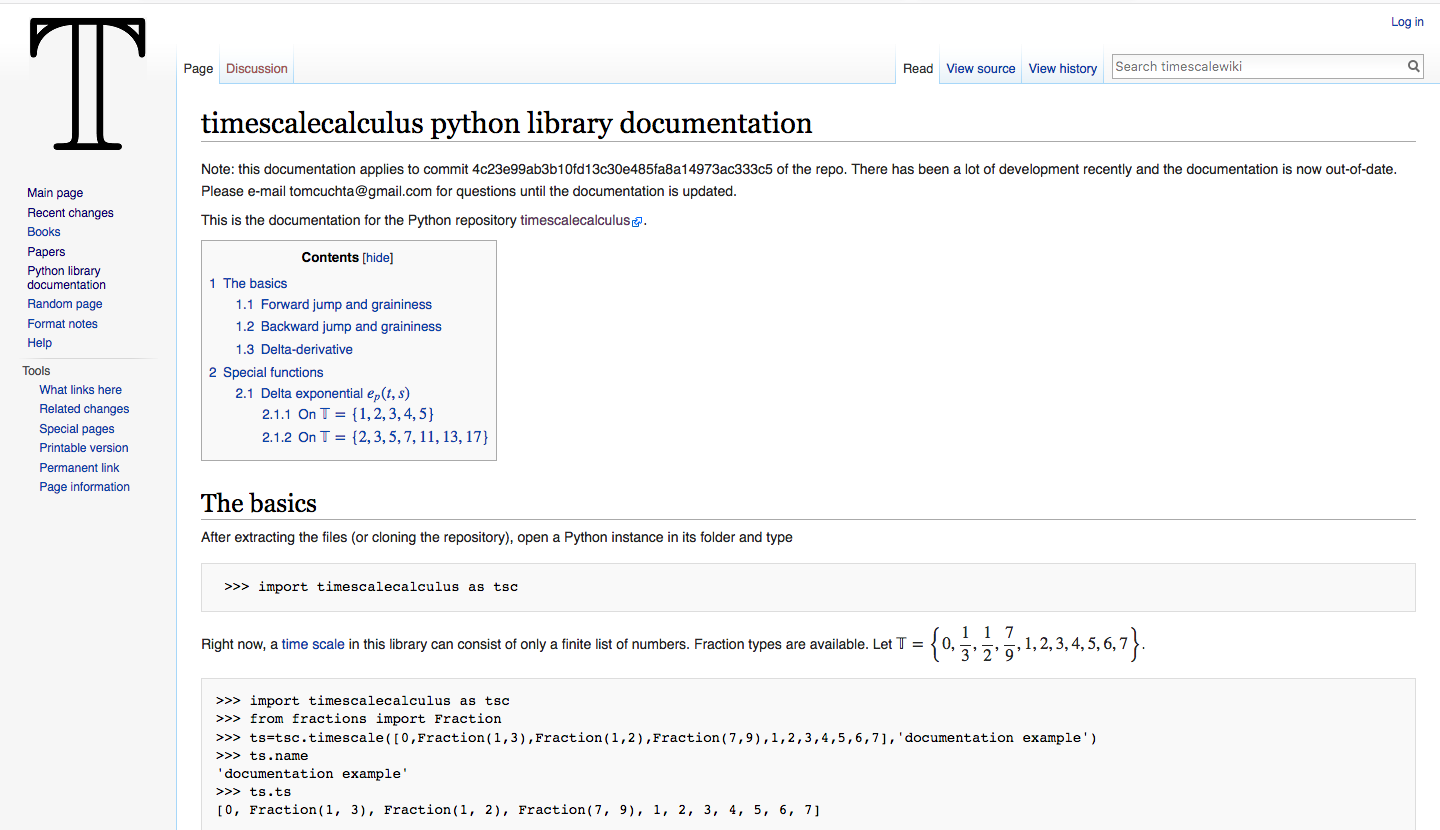
\includegraphics[width=\paperwidth]{doc}}
	\begin{frame}[plain]
	\end{frame}
}